\section{Smart Contract Security}
\label{sec:security}

Security was split on purpose: Member A built the controls in (roles, reentrancy guard, checks
effects interactions, pull payments, bounded pause), Member B secured the off chain trust boundary,
and Member C attacked the whole system, fixed what the attacks exposed and wrote this threat model.
The full documents are \code{docs/security/threat\_model.md} and \code{mitigation\_map.md}.

\subsection{Approach}
We listed the assets, the actors and how far each is trusted, drew the trust boundaries, and went
through each workflow with the STRIDE categories \cite{shostack2014}. Every threat that can be exercised
on a local chain became an attack test in \code{test/attacks/}: the attacker, the goal, the steps, and
what must still hold afterwards. The attack suite was then run on the code as handed over and on the
final code.

\begin{table}[H]
\centering\small
\caption{Assets}
\label{tab:assets}
\begin{tabularx}{\textwidth}{@{}P{0.9cm}P{4.2cm}L@{}}
\toprule
Id & Asset & Worst case if lost \\
\midrule
AS1 & Security deposits (vault) & Members lose their deposit; the group loses its cover \\
AS2 & Round contributions (circle) & A pot is stolen or stuck \\
AS3 & Credits (\code{withdrawable}) & A member cannot claim, or someone is paid twice \\
AS4 & Fair payout order & Someone picks the first slot, i.e. the interest free loan \\
AS5 & Reputation records & Honest members framed as defaulters and refused by circles \\
AS6 & Terms document & Members agree to terms other than the ones they see \\
AS7 & Liveness & A circle can neither finish nor refund: funds frozen \\
\bottomrule
\end{tabularx}
\end{table}

\begin{table}[H]
\centering\small
\caption{Actors and trust}
\label{tab:actors}
\begin{tabularx}{\textwidth}{@{}P{3.3cm}L@{}}
\toprule
Actor & Trusted for \\
\midrule
Member & Nothing: may default, collude, or be a smart contract. \\
Organizer & Nothing: never holds or moves money. \\
Platform admin & Not to abuse a bounded pause; cannot move money (Section~\ref{sec:admin}). \\
Deployer & The deployment transactions only; then renounces the module admin role (fix S3). \\
Keeper & Nothing: anyone may call the same functions. \\
Indexer, notifier, IPFS hosts & Nothing for correctness: the UI decides from the chain and re hashes the terms. \\
Block proposer & Not to grind the payout order (residual risk R1). \\
Token contract & To be a plain ERC20 without receiver hooks or blacklists (residual risk R2). \\
\bottomrule
\end{tabularx}
\end{table}

\paragraph{Trust boundaries.} (1) Chain and off chain: no off chain component can move money, and the
browser reads every value that decides an action from the contracts. (2) Factory registered circles and
everything else: the vault, draw and registry accept writes only from \code{CIRCLE\_ROLE} holders,
granted only by the factory, which only deploys clones of its own implementation. (3) One circle and
another: vault balances are keyed by (circle, member). (4) Members and the draw: commitments are bound
to the member's address and the shuffle entropy is fixed by the last reveal's block.

\subsection{Threats, controls and tests}
Status \textbf{Fixed} means the attack test failed on the code as handed over and passes now.

{\small
\begin{xltabular}{\textwidth}{@{}P{0.7cm}P{4.2cm}LP{1.0cm}P{1.6cm}@{}}
\caption{Threats, controls and the tests that prove them}\label{tab:threats}\\
\toprule
Id & Threat & Control & Test & Status \\
\midrule
\endfirsthead
\toprule
Id & Threat & Control & Test & Status \\
\midrule
\endhead
\bottomrule
\endfoot
T1 & Re enter a payout to be paid twice & \code{nonReentrant} on every entry point; effects before transfers; pull payments & A1 & Mitigated \\
T2 & Take the pot early and stop paying & deposit = 100\% of what is still owed; slashed each missed round & A2 & Mitigated \\
T3 & Join and never pay, in any slot & slash; uncovered misses repaid from the member's own pot first & A4 & Mitigated \\
T4 & Several members default together & pot of round $k$ covers debt and refill (Section~\ref{sec:invariant}) & A8 & Mitigated \\
T5 & Withhold a reveal to change the order or cancel the circle & removed, one contribution penalty shared by revealers; continues with 2 or more & A3 & Mitigated \\
T6 & Reveal last and finalize in one transaction, undo unless slot 1 & finalize only in a later block than the last reveal & A3 & \textbf{Fixed (S2)} \\
T7 & After revealing, finalize and undo until the order suits & entropy = hash of the last reveal's block & A3 & \textbf{Fixed (S2)} \\
T8 & Copy someone's commitment from the mempool & commitment bound to the member's address & A3 & Mitigated \\
T9 & Commit after seeing other secrets & no reveal before all commit or the window closes & A3 & Mitigated \\
T10 & A contract outside the factory slashes, releases, writes reputation or starts a draw & \code{CIRCLE\_ROLE} on every module write & A5 & Mitigated \\
T11 & A registered circle touches another circle's deposits & balances keyed by (circle, member) & A5 & Mitigated \\
T12 & Stolen deployer key registers a fake circle and frames members & deployer renounces the module admin role & A5 & \textbf{Fixed (S3)} \\
T13 & Organizer or admin takes the money & no function moves funds to them & A5 & Mitigated \\
T14 & Re initialize a clone or the implementation & \code{initializer}, factory only, same transaction & A5 & Mitigated \\
T15 & Admin pauses through a deadline: everyone slashed and recorded as defaulters & paused time is added to the round deadline & A6 & \textbf{Fixed (S1)} \\
T16 & Admin re pauses at once to freeze a circle & 7 day cooldown; each pause at most 7 days & A6 & \textbf{Fixed (S1)} \\
T17 & Settings that overflow packed storage & \code{initialize} rejects values that do not fit & A9 & Mitigated \\
T18 & A round too expensive to settle & \code{MAX\_MEMBERS} = 20; worst case 832,971 gas & A9 & Mitigated \\
T19 & Show members tampered terms & CID on chain; the UI re hashes the document & A7, B & Mitigated \\
T20 & Indexer lies or is down & decisions read the chain; chain fallback & B & Mitigated \\
T21 & Keeper stops & every keeper call is public & B & Mitigated \\
R1 & Proposer influence on the seed; prevrandao fallback after 256 blocks & none beyond S2 & -- & Residual \\
R2 & A hook or blacklist token blocks push refunds & token fixed to a plain ERC20 & A1 & Residual \\
R3 & Defaulter returns with a new address (Sybil) & the deposit is the protection & A4 & Residual \\
R4 & Bounded pause stays a small trust point & bounded, deadline extended, no funds trapped & A6 & Accepted \\
\end{xltabular}
}

\subsection{Attack scenarios}

\begin{table}[H]
\centering\small
\caption{Attack test scenarios (\code{npm run test:attacks}, 38 tests)}
\label{tab:attacks}
\begin{tabularx}{\textwidth}{@{}P{0.7cm}P{3.8cm}LP{0.8cm}@{}}
\toprule
Id & Scenario & What the test shows & Tests \\
\midrule
A1 & Payout reentrancy & A member contract on an ERC777 style hook token re enters \code{claimPayout}, \code{settleRound} and refunds: every attempt is refused by the guard, the attacker is paid exactly once, everyone ends whole. & 5 \\
A2 & Take the pot and run & For slots 1 to 3, honest members end exactly whole and the runner gains exactly nothing; the next strict circle refuses the runner. & 4 \\
A3 & Order rigging & Reveal and finalize at once is refused; the order is identical whoever finalizes and whenever; grinding never succeeds; withholding, copying and late commits fail. & 6 \\
A4 & Join and never pay & For every slot, honest members end whole, the free rider never ends ahead, nothing is stuck; walk away and Sybil variants. & 6 \\
A5 & Fake circles and privilege abuse & Outsider contracts, a compromised registered circle, the organizer, the admin and a stolen deployer key cannot move or misrecord anything; circles are exact clones. & 6 \\
A6 & Admin pause abuse & A pause through the deadline no longer causes defaults; an expired pause gives its time back; pauses cannot be chained; nothing is trapped. & 5 \\
A7 & Terms tampering & A one character change no longer matches the on chain CID. & 3 \\
A8 & Colluding defaulters & Invariants over 24 seeded random default patterns (200 also pass). & 1 \\
A9 & Limits and gas exhaustion & Oversized settings rejected; 20 member worst case far below the block limit. & 2 \\
\bottomrule
\end{tabularx}
\end{table}

\subsection{Vulnerabilities found and fixed}

\subsubsection{S1: an admin pause could force every member into default}
\label{sec:s1}
\textbf{Found by A6.} The pause blocked \code{contribute} but the round clock kept running, and
\code{settleRound} is (correctly) not blocked by a pause. An admin who paused an hour before a deadline
and stayed paused past it made it impossible for anyone to pay; then anyone could settle the round, and
every member was slashed one contribution and got a default on their public record. A pause that
expired could also be renewed in the same second, freezing the circle. On the handed over code the test
saw all four members slashed.

\textbf{Fix.} The base contract now records how long the circle has been paused, and the round deadline
adds the time paused during that round (Figure~\ref{fig:s1}); a new pause needs seven days of unpaused
time after the previous one ended. A round that had already closed before a pause can still be settled
during it, so a pause cannot help defaulters either.

\begin{figure}[H]
\centering
\begin{tikzpicture}[x=1cm,y=1cm, lb/.style={font=\scriptsize, align=center}]
\draw[-{Stealth}, thick] (0,0) -- (14,0) node[right, font=\scriptsize]{time};
\foreach \x/\t in {0.4/round starts, 6.6/pause, 8.0/old deadline, 10.6/unpause, 12.0/new deadline} {
  \draw (\x,0.15) -- (\x,-0.15) node[below, lb]{\t};
}
\fill[black!15] (6.6,0.22) rectangle (10.6,0.88);
\node[lb] at (9.33,0.55) {paused: nobody\\can pay (4 days)};
\draw[|<->|] (6.6,-0.95) -- node[below, lb]{1 hour left when paused} (8.0,-0.95);
\draw[|<->|] (10.6,-0.95) -- node[below, lb]{still 1 hour left} (12.0,-0.95);
\draw[densely dashed] (8.0,0) -- (8.0,1.15) node[above, lb]{before S1: anyone could settle here\\and every member was slashed};
\end{tikzpicture}
\caption{S1: the time spent paused is added to the payment deadline}
\label{fig:s1}
\end{figure}

\begin{lstlisting}[language=Solidity]
function pause() external onlyRole(PAUSER_ROLE) {
    _requireNotPaused();
    _closeExpiredPause();                 // books a pause that ran out by itself
    uint256 lastEnd = _lastPauseEnd;
    require(lastEnd == 0 || block.timestamp >= lastEnd + PAUSE_COOLDOWN, "Lifecycle: pause cooldown");
    _pause();
    _pausedAt = uint40(block.timestamp);
    _pauseExpiresAt = uint40(block.timestamp + MAX_PAUSE_DURATION);
}
// Circle
function roundDeadline() public view returns (uint256) {
    return uint256(_roundStart) + _roundDuration + _gracePeriod + (totalPausedTime() - _roundPauseMark);
}
\end{lstlisting}

\subsubsection{S2: the last revealer could choose its payout slot}
\label{sec:s2}
\textbf{Found by A3.} The baseline mixed \code{block.prevrandao} into the seed at finalize time
\cite{eip4399}, and anyone may finalize. A member that is a smart contract could therefore (a) send the
last reveal and \code{finalizeDraw} in one transaction, check its position, and revert both unless it got
slot 1, retrying every block until lucky; or (b) after revealing normally, call \code{finalizeDraw},
check, and revert, block after block, until the order suited it. On the handed over code the grinding
attacker obtained the slot it wanted within twelve blocks.

\textbf{Fix.} \code{reveal} records the block number; \code{finalize} must run in a later block, and the
entropy is the hash of the block that holds the last reveal (Figure~\ref{fig:s2}). The member who sends
the last reveal cannot know that hash when signing, and once the block exists the order is the same for
every finalize call, so retrying gains nothing. The test finalizes in the next block, rolls the chain
back, finalizes 26 blocks and a day later from another account, and gets the identical order.

\begin{figure}[H]
\centering
\begin{tikzpicture}[blk/.style={draw=boxline, minimum width=1.9cm, minimum height=0.8cm, font=\scriptsize, align=center},
  lb/.style={font=\scriptsize, align=center}]
\node[blk] (b1) at (0,0) {block $N-1$\\reveals};
\node[blk, line width=1pt] (b2) at (2.4,0) {block $N$\\last reveal};
\node[blk] (b3) at (4.8,0) {block $N+1$};
\node[blk] (b4) at (7.2,0) {\dots};
\node[blk] (b5) at (9.6,0) {block $N+k$\\finalize};
\draw[-{Stealth}] (b1) -- (b2); \draw[-{Stealth}] (b2) -- (b3); \draw[-{Stealth}] (b3) -- (b4); \draw[-{Stealth}] (b4) -- (b5);
\node[lb, below=0.35cm of b2] (h) {$H_N$ = hash of block $N$\\unknown when the reveal is sent};
\node[lb, below=0.35cm of b5] (s) {seed = keccak(secrets, $H_N$, circle)\\same for every $k \geq 1$};
\draw[-{Stealth}, densely dashed] (h) -- (s);
\node[lb, above=0.25cm of b2] {finalize in block $N$ refused};
\end{tikzpicture}
\caption{S2: the payout order is fixed by the block that holds the last reveal}
\label{fig:s2}
\end{figure}

\begin{lstlisting}[language=Solidity]
uint256 lastReveal = d.lastRevealBlock;
require(block.number > lastReveal, "Order: finalize in a later block");
bytes32 entropy = lastReveal == 0 ? bytes32(0) : blockhash(lastReveal);
if (entropy == bytes32(0)) entropy = bytes32(block.prevrandao); // nobody revealed, or > 256 blocks old
bytes32 seed = keccak256(abi.encodePacked(d.seed, entropy, msg.sender));
\end{lstlisting}

\subsubsection{S3: the deployer kept a role it no longer needed}
\textbf{Found by A5.} The deploying account kept \code{DEFAULT\_ADMIN\_ROLE} on the vault, the draw and
the registry. If that key were stolen, the thief could grant itself \code{REGISTRAR\_ROLE}, register a
fake circle and write false defaults into anyone's reputation (vault balances stay safe because they are
keyed by circle). \textbf{Fix:} the deploy script renounces the role once the factory is registered, so
the set of registrars is fixed forever. The test deploys with the real script and shows that even the
deployer can no longer register anything.

\subsubsection{Evidence}
\begin{table}[H]
\centering\small
\caption{Attack suite on the code as handed over and on the final code}
\label{tab:beforeafter}
\begin{tabular}{@{}lrr@{}}
\toprule
 & Handed over (A1 to A7) & Final (A1 to A9) \\
\midrule
Passing & 27 & 38 \\
Failing & 8 (3 pause, 3 draw, 1 admin role, 1 clone check) & 0 \\
\bottomrule
\end{tabular}
\end{table}
The clone check failed only because clones did not exist before optimization G1. Full outputs are in
\code{docs/security/attack\_results\_baseline.txt} and \code{attack\_results\_final.txt}.

\subsection{Why colluding defaulters cannot leave the group short}
\label{sec:invariant}
Member A's handoff warned that if several members with empty deposits miss payments in the same
rounds, a shortfall might remain. We checked whether it can last. Consider the settlement of round $k$.
The $k-1$ members already paid out each contribute $c$ to the pot, either by paying or through a slash
that their deposit always covers in full, so the pot is at least $(k-1)c$. The recipient missed $m \le
k-1$ rounds before its payout; of those, $s$ were slashed from its deposit and $mc-s$ became debt.
Repaying the debt and refilling the deposit needs $(mc - s) + s = mc \le (k-1)c$, which the pot always
covers. Hence after every payout the recipient owes nothing and is again 100\% covered, so nobody can
still owe money when the circle completes. Attack test A8 checks exactly this over 24 seeded random
default patterns with 4 and 5 members (and 200 more with another seed): after each payout the recipient
has no debt and its deposit equals $(N-k)c$; at the end there is no debt, no deficit, no locked deposit
and no token left in the circle; money is conserved; honest members end exactly whole and nobody ends
ahead. A consequence is that the leftover debt branch in \code{\_complete} is never reached; it stays as
a defensive fallback.

\subsection{Off chain trust}
The browser downloads the terms by CID, hashes them with Web Crypto and compares the result with the
CID stored on chain (Figure~\ref{fig:terms}). When the indexer stops answering, the app switches to
reading lists, history and reminders from the chain (Figure~\ref{fig:offline}).

\begin{figure}[H]
\centering
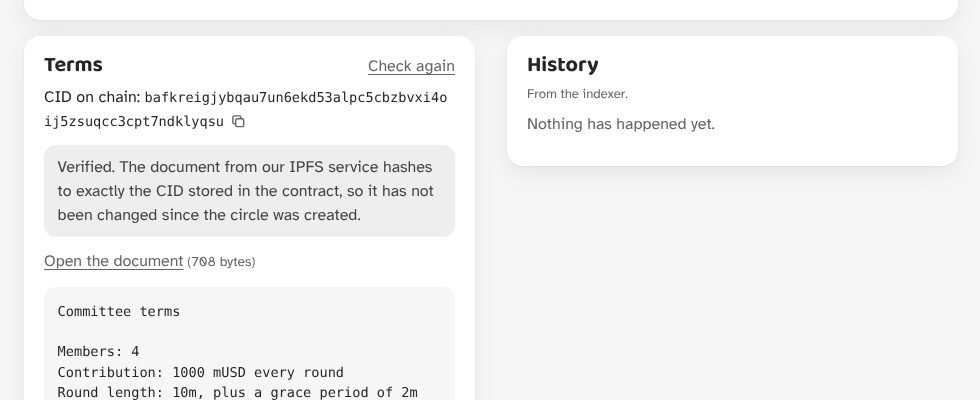
\includegraphics[width=0.48\textwidth]{figures/shot_terms_verified.jpg}\hfill
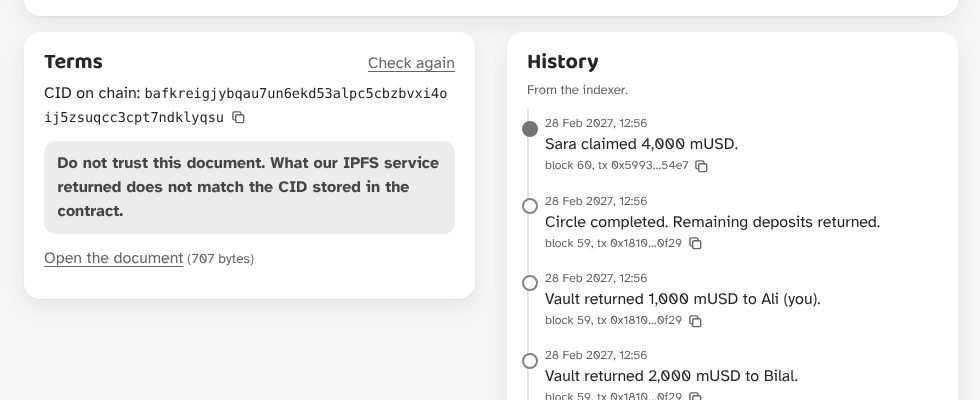
\includegraphics[width=0.48\textwidth]{figures/shot_tampered_terms.jpg}
\caption{Terms check: original document verified (left), tampered document refused (right)}
\label{fig:terms}
\end{figure}

\begin{figure}[H]
\centering
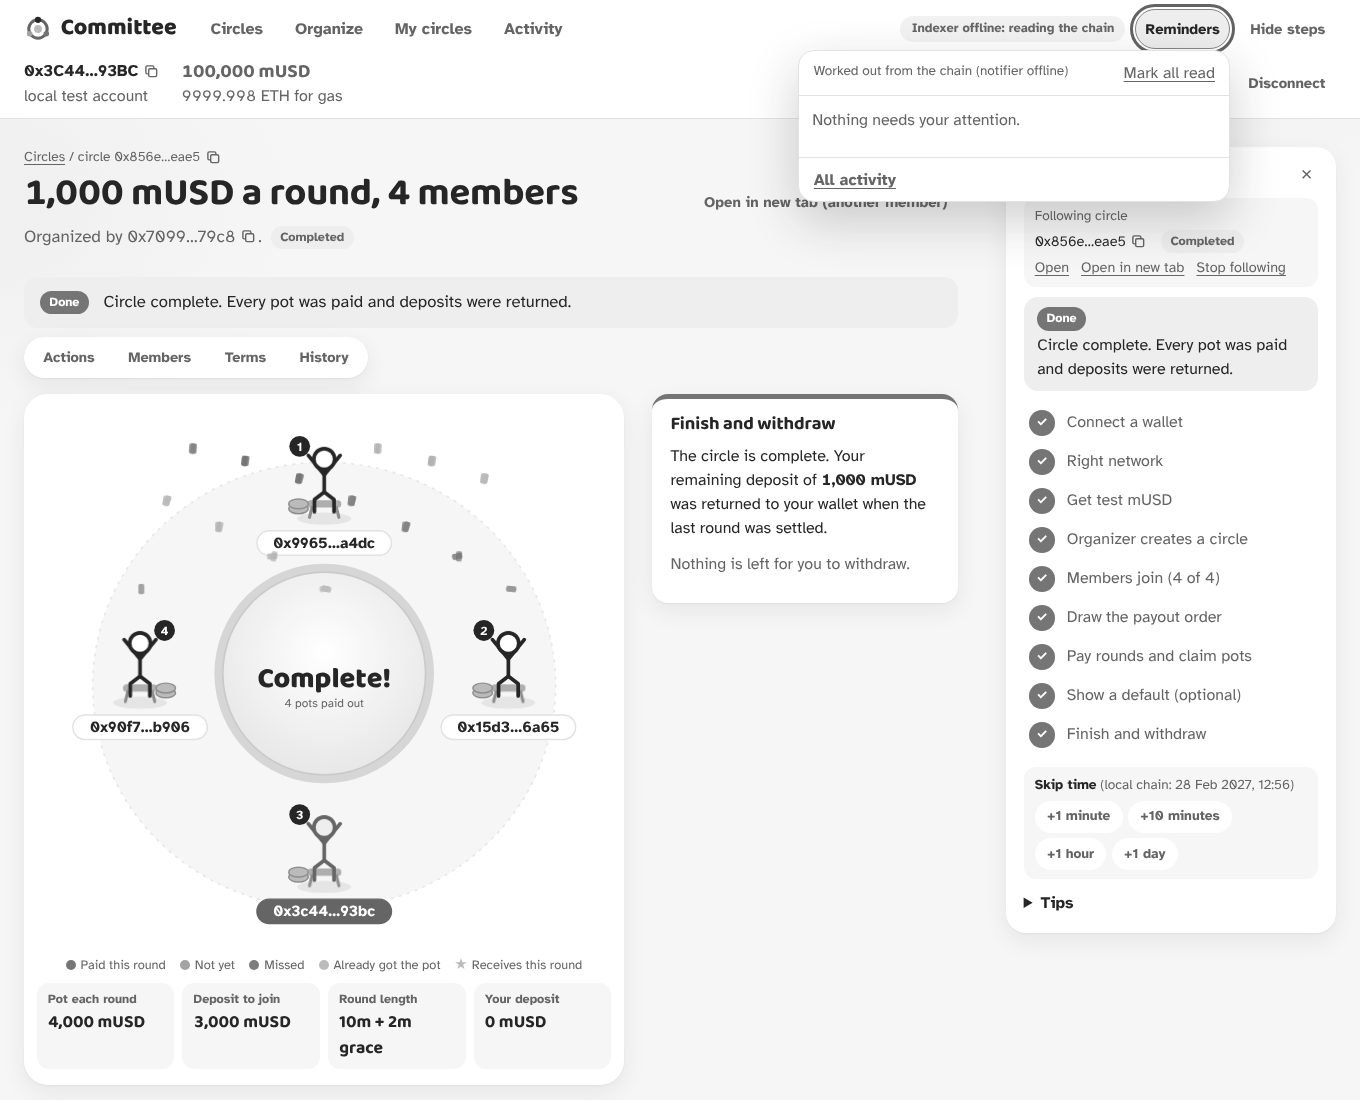
\includegraphics[width=0.8\textwidth]{figures/shot_indexer_offline.jpg}
\caption{Indexer stopped: the app reads the chain directly and keeps working}
\label{fig:offline}
\end{figure}

\subsection{Who is the admin, and what can they do?}
\label{sec:admin}
The admin is the account that deploys the system, i.e. the platform operator. After fix S3 it keeps one
power: \code{PAUSER\_ROLE} on each circle, which stops \code{join} and \code{contribute}. A pause lasts at
most seven days and ends by itself; the paused time is added to the payment deadline, so nobody misses a
payment because of it; the next pause is possible only seven days after the previous one ended, so a
circle is unpaused at least half of the time; settling closed rounds, claiming, finalizing the draw and
cancel refunds keep working. The admin has no function that moves tokens. Figure~\ref{fig:pauseui} shows
the live app refusing a second pause.

\begin{figure}[H]
\centering
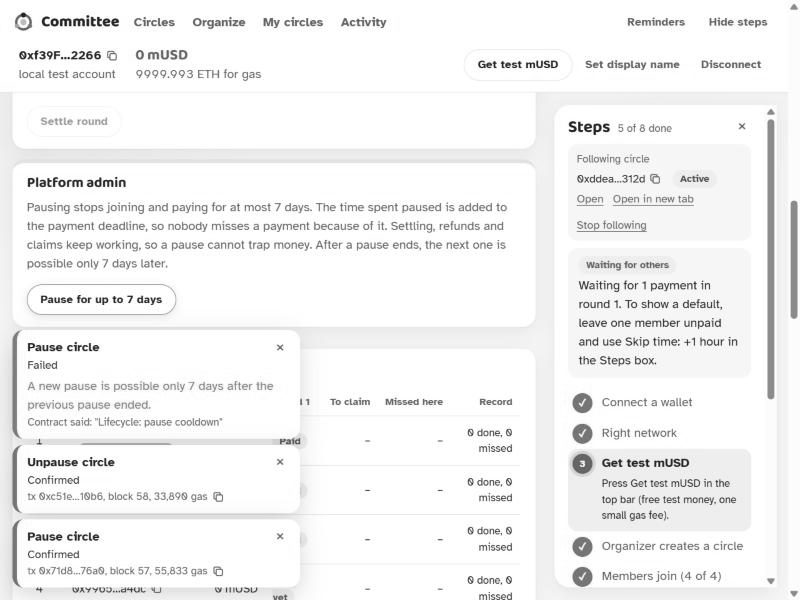
\includegraphics[width=0.62\textwidth]{figures/shot_pause_cooldown.jpg}
\caption{Live check of S1: pause and unpause confirmed, an immediate second pause refused with a plain message}
\label{fig:pauseui}
\end{figure}

\subsection{Residual risks}
\begin{itemize}
  \item \textbf{R1, randomness.} A block proposer who is also a member could still influence the hash of
        the block holding the last reveal by choosing what to include. If finalize happens more than 256
        blocks after the last reveal (possible when some members never reveal), \code{blockhash} returns
        zero and the seed falls back to \code{prevrandao}, which a contract caller could grind again.
        Chainlink VRF \cite{chainlinkvrf} removes both.
  \item \textbf{R2, token assumption.} Deposits are refunded by pushing tokens in a loop. With a plain ERC20
        this cannot fail, and the token is fixed at deployment; a token with blacklists or receiver hooks
        would let one member block refunds, which A1 demonstrates with a hook token. A production
        deployment on such a token should switch to pull withdrawals.
  \item \textbf{R3, Sybil.} Reputation is per address, so a defaulter can return with a new address. This is
        acceptable because the deposit, not the score, protects the group (A2, A4, A8).
  \item \textbf{R4, pause.} The bounded pause remains a small trust point by design.
\end{itemize}
